% Slide deck for the dissertation. Compile from this folder:
%   latexmk -pdf presentation.tex
% Title, author and supervisors come from ../config/metadata.tex.
\documentclass[aspectratio=169,11pt]{beamer}

% Everything that identifies the thesis lives here.
% The covers and title pages are built from these values.
\newcommand{\thesisyear}{2026}
\newcommand{\thesisdate}{October 2026}
\newcommand{\thesisauthor}{Dumilde José de Matos}
\newcommand{\thesistitle}{EEG-Based Remote Car Control Using the Emotiv EPOC X: System Development and Experimental Evaluation}
\newcommand{\thesiscovertitle}{EEG-Based Remote Car Control\\Using the Emotiv EPOC X:} % Line breaks used on the cover.
\newcommand{\thesiscoversubtitle}{System Development\\and Experimental Evaluation}
\newcommand{\thesisdegree}{Creative Computing and Artificial Intelligence}
\newcommand{\thesisdegreecover}{MASTER’S IN CREATIVE COMPUTING\\AND ARTIFICIAL INTELLIGENCE}
\newcommand{\thesissupervisorscover}{Prof. Dr. Pamela Teubig\\Prof. Dr. José Graça}
\newcommand{\thesissupervision}{Doutora Pamela Teubig, professora assistente do \textit{IADE} e de Doutor José Graça, professor do IADE}
\newcommand{\thesisinstitution}{IADE - Faculdade de Design, Tecnologia e Comunicação da Universidade Europeia}
\newcommand{\thesisinstitutioncover}{IADE, Faculdade de Design, Tecnologia e Comunicação\\da Universidade Europeia}
\newcommand{\thesisformcode}{MOD-195.IADEV02;  07-07-2023} % Margin of the opening pages.
\newcommand{\thesiscovercode}{MOD.IADE-315/V01-EN;  05-05-2023} % Edge of the back cover.

\graphicspath{{../figures/}{../figures/logos/}}

\usepackage[T1]{fontenc}
\usepackage[english]{babel}
\usepackage[sfdefault]{roboto}
\usepackage{booktabs}
\usepackage{tabularx}
\usepackage{amsmath}
\usepackage{tikz}
\usetikzlibrary{arrows.meta,positioning,shapes.geometric,fit,calc}

% --- Theme ---
\definecolor{ink}{HTML}{1B2A41}
\definecolor{accent}{HTML}{0F6E8C}
\definecolor{accentlight}{HTML}{E3F1F5}
\definecolor{muted}{HTML}{6B7785}
\definecolor{warn}{HTML}{B5651D}
\definecolor{warnlight}{HTML}{FBF0E4}

\setbeamercolor{normal text}{fg=ink,bg=white}
\setbeamercolor{structure}{fg=accent}
\setbeamercolor{frametitle}{fg=ink}
\setbeamercolor{title}{fg=white}
\setbeamercolor{item}{fg=accent}
\setbeamercolor{block title}{fg=white,bg=accent}
\setbeamercolor{block body}{fg=ink,bg=accentlight}
\setbeamerfont{frametitle}{size=\Large,series=\bfseries}
\setbeamerfont{block title}{series=\bfseries}
\setbeamertemplate{navigation symbols}{}
\setbeamertemplate{itemize items}{\raisebox{.15em}{\tiny$\blacksquare$}}
\setbeamertemplate{enumerate items}[default]
\setbeamertemplate{blocks}[rounded][shadow=false]
\setlength{\leftmargini}{1.2em}

\setbeamertemplate{frametitle}{%
  \vspace*{.6em}%
  \begin{beamercolorbox}[wd=\paperwidth,leftskip=1.2em]{frametitle}
    {\usebeamerfont{frametitle}\insertframetitle}\par
    \ifx\insertframesubtitle\empty\else
      {\small\color{muted}\insertframesubtitle}\par
    \fi
  \end{beamercolorbox}%
  \vspace*{-.4em}\hspace*{1.2em}{\color{accent}\rule{2.2em}{2pt}}%
}

\setbeamertemplate{footline}{%
  \leavevmode\hbox to \paperwidth{%
    \hspace{1.2em}{\tiny\color{muted}\thesisauthor\ \textbullet\ \thesisdegree}%
    \hfill
    {\tiny\color{muted}\insertsection}\hspace{1.5em}%
    {\tiny\color{accent}\bfseries\insertframenumber}\hspace{1.2em}}%
  \vspace{.8em}}

% Section divider slides.
\AtBeginSection{%
  \begingroup
  \setbeamertemplate{footline}{}
  \setbeamercolor{background canvas}{bg=ink}
  \begin{frame}[plain,noframenumbering]
    \vfill
    \hspace*{1.5em}{\color{accent!60}\Large\bfseries\secnum}\par\medskip
    \hspace*{1.5em}{\color{white}\huge\bfseries\insertsectionhead}\par
    \vfill
  \end{frame}
  \endgroup
}
\newcommand{\secnum}{\ifcase\value{section}\or 01\or 02\or 03\or 04\or 05\or 06\or 07\fi}

% Box for content that is still to be filled in once results exist.
% Optional argument: minimum height, e.g. \pending[3.5cm]{...} for a chart slot.
\newcommand{\pending}[2][0pt]{%
  \begin{tikzpicture}
    \node[draw=warn,dashed,fill=warnlight,rounded corners=3pt,text width=.92\linewidth,
          minimum height=#1,align=center,inner sep=8pt,font=\small,text=warn]{#2};
  \end{tikzpicture}}

\title{\thesistitle}
\author{\thesisauthor}
\date{\thesisdate}

\begin{document}

% ------------------------------------------------------------------ Title
{
\setbeamertemplate{footline}{}
\setbeamercolor{background canvas}{bg=ink}
\begin{frame}[plain]
  \begin{tikzpicture}[remember picture,overlay]
    \fill[accent] (current page.north west) rectangle ([xshift=.5em]current page.south west);
    \node[anchor=north east,fill=white,inner sep=6pt,rounded corners=2pt]
      at ([xshift=-1.5em,yshift=-1.5em]current page.north east)
      {
\includegraphics[height=1.1em]{logo-iade-faculdade.png}};
  \end{tikzpicture}
  \vspace{2.5em}
  {\color{accent!55}\small\bfseries\MakeUppercase{Master's Dissertation}}\par\medskip
  {\color{white}\LARGE\bfseries EEG-Based Remote Car Control\\Using the Emotiv EPOC X\par}
  \medskip
  {\color{white!75}\large System Development and Experimental Evaluation\par}
  \vspace{2.2em}
  {\color{white}\bfseries\thesisauthor}\par
  {\color{white!70}\small \thesisdegree}\par\medskip
  {\color{white!70}\footnotesize Supervisors: Prof.\ Dr.\ Pamela Teubig \textbullet\ Prof.\ Dr.\ José Graça}\par
  {\color{white!70}\footnotesize \thesisdate}
\end{frame}
}

% ------------------------------------------------------------------ Outline
\begin{frame}{Outline}
  \begin{columns}[T]
    \begin{column}{.48\textwidth}
      \begin{enumerate}
        \item Introduction
        \item BCI \& EEG: Literature Review
        \item The Brain-Controlled Car System
        \item Methodology \& Evaluation
      \end{enumerate}
    \end{column}
    \begin{column}{.48\textwidth}
      \begin{enumerate}\setcounter{enumi}{4}
        \item Results
        \item Discussion
        \item Conclusion \& Future Work
      \end{enumerate}
    \end{column}
  \end{columns}
\end{frame}

% ================================================================== 1
\section{Introduction}

\begin{frame}{Background and Context}
  \begin{columns}[T]
    \begin{column}{.55\textwidth}
      \begin{itemize}
        \item A \textbf{brain-computer interface (BCI)} turns brain activity into commands for an external device, without muscle movement.
        \item \textbf{Non-invasive EEG} records that activity from the scalp, with no surgery.
        \item \textbf{Consumer headsets} such as the Emotiv EPOC X have made EEG cheap and portable.
        \item Controlling \textbf{vehicles and robots} is a demanding test: commands must be correct, fast and safe.
      \end{itemize}
    \end{column}
    \begin{column}{.4\textwidth}
      \begin{block}{Study platform}
        \textbf{Emotiv EPOC X} headset\\
        Purpose-built \textbf{remote car}\\
        Open-source \textbf{Python framework} linking the two
      \end{block}
    \end{column}
  \end{columns}
\end{frame}

\begin{frame}{Motivation}
  \begin{columns}[T]
    \begin{column}{.48\textwidth}
      \begin{block}{Real need}
        Hands-free and assistive control for people who cannot rely on conventional input.
      \end{block}
      \medskip
      \begin{block}{Lower cost}
        Consumer EEG hardware puts BCI research within reach of small labs and individuals.
      \end{block}
    \end{column}
    \begin{column}{.48\textwidth}
      \begin{block}{Missing tooling}
        There is little open, reproducible software for connecting consumer EEG to physical devices.
      \end{block}
      \medskip
      \begin{block}{Open question}
        It is still unclear how dependable consumer EEG is for real-time physical control.
      \end{block}
    \end{column}
  \end{columns}
\end{frame}

\begin{frame}{Problem Statement and Research Gap}
  \begin{itemize}
    \item Mental commands from consumer EEG are \textbf{noisy} and \textbf{vary between users}.
    \item Driving a physical car needs commands that are \textbf{dependable}, \textbf{timely} and \textbf{safe}.
    \item It is unclear how far the EPOC X meets those demands.
  \end{itemize}
  \bigskip
  \begin{block}{Research gap}
    Few studies offer an \textbf{open framework} and report \textbf{reliability and latency together} on a \textbf{physical vehicle}.
  \end{block}
\end{frame}

\begin{frame}{Research Question and Objective}
  \vspace{.5em}
  \begin{block}{Research question}
    \large To what extent can mental commands from the Emotiv EPOC X, processed by an open-source Python framework, reliably control a remote car in real time?
  \end{block}
  \bigskip
  \begin{block}{Main objective}
    To design, build and experimentally evaluate a brain-controlled car system, driven by Emotiv EPOC X mental commands through an open-source Python framework.
  \end{block}
\end{frame}

\begin{frame}{Specific Objectives}
  \small
  \begin{columns}[T]
    \begin{column}{.48\textwidth}
      \begin{enumerate}
        \item \textbf{Review} the literature on BCI and EEG control \hfill{\color{muted}Ch.\,2}
        \item \textbf{Build} the car and its electronics \hfill{\color{muted}Ch.\,3}
        \item \textbf{Develop} the Python framework and integrate it with the car \hfill{\color{muted}Ch.\,3}
        \item \textbf{Add} safety mechanisms \hfill{\color{muted}Ch.\,3}
      \end{enumerate}
    \end{column}
    \begin{column}{.48\textwidth}
      \begin{enumerate}\setcounter{enumi}{4}
        \item \textbf{Define} the protocol and metrics \hfill{\color{muted}Ch.\,4}
        \item \textbf{Run} the experiments \hfill{\color{muted}Ch.\,4}
        \item \textbf{Analyse} the results \hfill{\color{muted}Ch.\,5--6}
        \item \textbf{Publish} the code as open source \hfill{\color{muted}App.}
      \end{enumerate}
    \end{column}
  \end{columns}
\end{frame}

\begin{frame}{Hypotheses and Scope}
  \begin{columns}[T]
    \begin{column}{.5\textwidth}
      \textbf{Hypotheses}\par\smallskip
      \begin{itemize}
        \item[\color{accent}\bfseries H1] Command success rate reaches a set threshold.
        \item[\color{accent}\bfseries H2] End-to-end response time stays within a set limit.
        \item[\color{accent}\bfseries H3] Performance changes across sessions.
      \end{itemize}
      \medskip
      \pending{Thresholds to be set from the literature and the pilot study.}
    \end{column}
    \begin{column}{.45\textwidth}
      \textbf{In scope}\par\smallskip
      \begin{itemize}
        \item One headset, Emotiv's built-in detection
        \item One purpose-built car
        \item Controlled indoor environment
      \end{itemize}
      \medskip
      \textbf{Out of scope}\par\smallskip
      \begin{itemize}
        \item Clinical users
        \item Real road use
      \end{itemize}
    \end{column}
  \end{columns}
\end{frame}

% ================================================================== 2
\section{BCI \& EEG: Literature Review}

\begin{frame}{Topics Covered}
  \begin{columns}[T]
    \begin{column}{.48\textwidth}
      \begin{itemize}
        \item Fundamentals of brain-computer interfaces
        \item EEG technology and signal acquisition
        \item EEG-based BCI paradigms
        \item Emotiv EPOC X: architecture and capabilities
        \item Emotiv mental commands: principles and limits
      \end{itemize}
    \end{column}
    \begin{column}{.48\textwidth}
      \begin{itemize}
        \item Consumer-grade EEG in BCI applications
        \item Machine learning for EEG classification
        \item EEG control of vehicles and mobile robots
        \item Safety and reliability in BCI systems
        \item Existing frameworks and related work
      \end{itemize}
    \end{column}
  \end{columns}
\end{frame}

\begin{frame}{Challenges of Real-Time BCI Control}
  \begin{columns}[T]
    \begin{column}{.48\textwidth}
      \begin{block}{Detection reliability}
        Classifying intent correctly from a noisy, low-resolution signal.
      \end{block}
      \medskip
      \begin{block}{Response latency}
        Delay between intention and action limits real-time control.
      \end{block}
    \end{column}
    \begin{column}{.48\textwidth}
      \begin{block}{False and missed commands}
        Unintended activations are a safety risk; misses frustrate the user.
      \end{block}
      \medskip
      \begin{block}{Workload and adaptation}
        Sustained concentration is tiring; users and models both need to adapt.
      \end{block}
    \end{column}
  \end{columns}
\end{frame}

% ================================================================== 3
\section{The Brain-Controlled Car System}

\begin{frame}{System Requirements}
  \begin{columns}[T]
    \begin{column}{.48\textwidth}
      \textbf{Functional}\par\smallskip
      \begin{itemize}
        \item[\color{accent}\bfseries FR1] Acquire mental commands from the headset
        \item[\color{accent}\bfseries FR2] Map commands to car actions
        \item[\color{accent}\bfseries FR3] Drive the car wirelessly
        \item[\color{accent}\bfseries FR4] Stop on demand
        \item[\color{accent}\bfseries FR5] Log every session
      \end{itemize}
    \end{column}
    \begin{column}{.48\textwidth}
      \textbf{Non-functional}\par\smallskip
      \begin{itemize}
        \item[\color{accent}\bfseries NFR1] Low latency
        \item[\color{accent}\bfseries NFR2] Reliability
        \item[\color{accent}\bfseries NFR3] Safety by default
        \item[\color{accent}\bfseries NFR4] Portability and openness
      \end{itemize}
    \end{column}
  \end{columns}
\end{frame}

\begin{frame}{Overall Architecture}
  \centering
  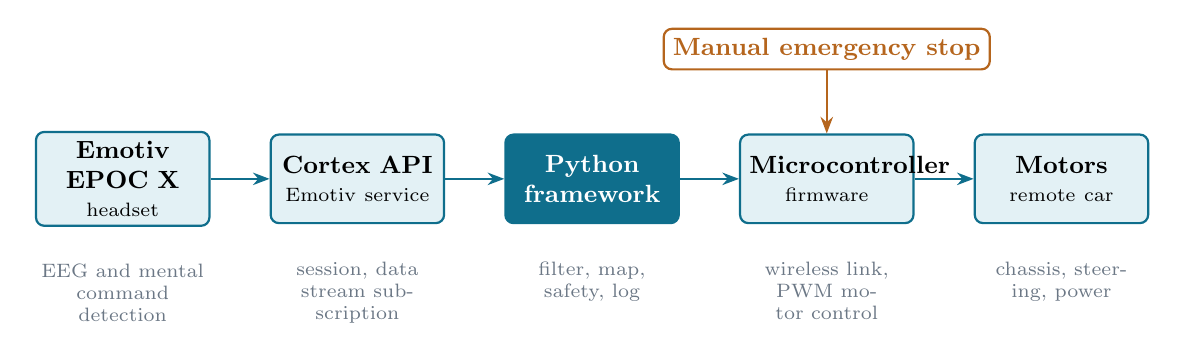
\begin{tikzpicture}[
      box/.style={draw=accent,fill=accentlight,rounded corners=3pt,thick,
                  minimum height=3.2em,text width=5.6em,align=center,font=\small},
      sub/.style={font=\scriptsize,text=muted,align=center,text width=6.2em},
      arr/.style={-{Stealth[length=6pt]},thick,accent},
      node distance=.75cm]
    \node[box] (h) {\textbf{Emotiv EPOC X}\\[-1pt]{\scriptsize headset}};
    \node[box,right=of h] (c) {\textbf{Cortex API}\\[-1pt]{\scriptsize Emotiv service}};
    \node[box,right=of c,fill=accent,text=white] (p) {\textbf{Python framework}};
    \node[box,right=of p] (m) {\textbf{Microcontroller}\\[-1pt]{\scriptsize firmware}};
    \node[box,right=of m] (car) {\textbf{Motors}\\[-1pt]{\scriptsize remote car}};
    \draw[arr] (h) -- (c);
    \draw[arr] (c) -- (p);
    \draw[arr] (p) -- (m);
    \draw[arr] (m) -- (car);
    \node[sub,below=.35cm of h]   {EEG and mental command detection};
    \node[sub,below=.35cm of c]   {session, data stream subscription};
    \node[sub,below=.35cm of p]   {filter, map, safety, log};
    \node[sub,below=.35cm of m]   {wireless link, PWM motor control};
    \node[sub,below=.35cm of car] {chassis, steering, power};
    \node[draw=warn,thick,rounded corners=3pt,font=\small,text=warn,above=.8cm of m]
         (e) {\textbf{Manual emergency stop}};
    \draw[arr,warn] (e) -- (m);
  \end{tikzpicture}
  \vspace{1em}

  \small Modular design: each stage can be tested or replaced on its own.
\end{frame}

\begin{frame}{From Mental Command to Car Movement}
  \begin{columns}[T]
    \begin{column}{.5\textwidth}
      \textbf{Command processing}\par\smallskip
      \begin{enumerate}
        \item Receive action and power value from Cortex
        \item Timestamp on arrival
        \item Discard commands below a power threshold
        \item Debounce: command must persist before it acts
        \item Map to a car action and send to the car
      \end{enumerate}
    \end{column}
    \begin{column}{.45\textwidth}
      \textbf{Example mapping}\par\smallskip
      \begin{tabular}{@{}ll@{}}
        \toprule
        Mental command & Car action \\
        \midrule
        Push    & Forward \\
        Neutral & Stop \\
        Left / Right & Steer \\
        \bottomrule
      \end{tabular}
      \medskip

      {\footnotesize\color{muted}Neutral is the default state. Conflicting commands resolve to stop.}
    \end{column}
  \end{columns}
\end{frame}

\begin{frame}{Real-Time Control and Safety}
  \begin{columns}[T]
    \begin{column}{.48\textwidth}
      \begin{itemize}
        \item \textbf{Default to stopped} at start-up and on any error
        \item \textbf{Manual emergency stop}, independent of the EEG channel
        \item \textbf{Watchdog timeout}: the car stops if the signal or link is lost
        \item \textbf{Stale command rejection} in the control loop
        \item \textbf{Speed limits} in firmware
      \end{itemize}
    \end{column}
    \begin{column}{.48\textwidth}
      \begin{block}{Logging and monitoring}
        Timestamps, commands, power values and car actions recorded per session, with pseudonymised IDs.\\[.4em]
        Live view of signal quality, connection and car state.
      \end{block}
    \end{column}
  \end{columns}
\end{frame}

\begin{frame}{Technical Testing and Validation}
  \begin{itemize}
    \item \textbf{Unit tests} of framework modules
    \item \textbf{Bench tests} of motors and firmware
    \item \textbf{Integration tests} from framework to car
    \item \textbf{Simulated command source}, for testing without a headset
    \item \textbf{Timing and emergency stop tests}
  \end{itemize}
  \medskip
  \pending{Requirements-to-tests table (FR/NFR vs.\ outcome) to be added when testing is complete.}
\end{frame}

% ================================================================== 4
\section{Methodology \& Evaluation}

\begin{frame}{Research Design}
  \begin{columns}[T]
    \begin{column}{.48\textwidth}
      \begin{itemize}
        \item \textbf{Quantitative experimental} evaluation
        \item \textbf{Repeated measures}: each participant across several sessions
        \item \textbf{Controlled} indoor environment with consistent conditions
      \end{itemize}
    \end{column}
    \begin{column}{.48\textwidth}
      \begin{block}{Participants and ethics}
        Informed consent, GDPR-compliant data handling, pseudonymisation and the right to withdraw.
      \end{block}
      \smallskip
      \pending{Number of participants and ethics approval status to be confirmed.}
    \end{column}
  \end{columns}
\end{frame}

\begin{frame}{Experimental Procedure}
  \centering
  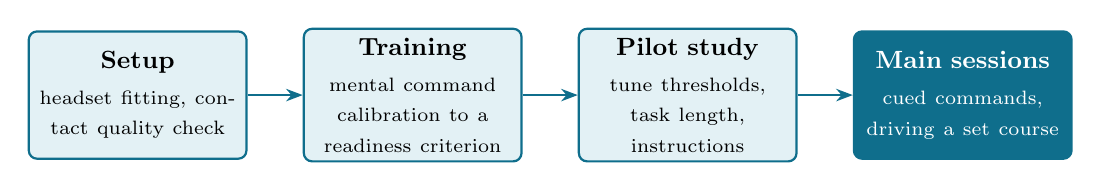
\begin{tikzpicture}[
      stage/.style={draw=accent,fill=accentlight,rounded corners=3pt,thick,
                   minimum height=4.6em,text width=7.2em,align=center,font=\small},
      arr/.style={-{Stealth[length=6pt]},thick,accent},
      node distance=.7cm]
    \node[stage] (a) {\textbf{Setup}\\[2pt]{\scriptsize headset fitting, contact quality check}};
    \node[stage,right=of a] (b) {\textbf{Training}\\[2pt]{\scriptsize mental command calibration to a readiness criterion}};
    \node[stage,right=of b] (c) {\textbf{Pilot study}\\[2pt]{\scriptsize tune thresholds, task length, instructions}};
    \node[stage,right=of c,fill=accent,text=white] (d) {\textbf{Main sessions}\\[2pt]{\scriptsize cued commands, driving a set course}};
    \draw[arr] (a) -- (b);
    \draw[arr] (b) -- (c);
    \draw[arr] (c) -- (d);
  \end{tikzpicture}
  \vspace{1.5em}

  \begin{columns}[T]
    \begin{column}{.45\textwidth}
      \begin{block}{Task 1: Cued commands}
        Single commands on a timed cue.
      \end{block}
    \end{column}
    \begin{column}{.45\textwidth}
      \begin{block}{Task 2: Course driving}
        Drive the car along a set course.
      \end{block}
    \end{column}
  \end{columns}
\end{frame}

\begin{frame}{Evaluation Metrics}
  \small
  \renewcommand{\arraystretch}{1.25}
  \begin{tabularx}{\textwidth}{@{}lXl@{}}
    \toprule
    \textbf{Metric} & \textbf{Definition} & \textbf{Unit} \\
    \midrule
    Command success rate   & Correct commands executed / commands cued & \% \\
    False activation rate  & Commands detected when none (or another) was intended & \% or /min \\
    Missed command rate    & Cued commands not detected in the time window & \% \\
    Detection latency      & Cue $\rightarrow$ detection by the framework & ms \\
    End-to-end response    & Cue $\rightarrow$ physical car response & ms \\
    Task completion rate   & Tasks finished / tasks attempted & \% \\
    Session variation      & Change in the metrics above across sessions & -- \\
    \bottomrule
  \end{tabularx}
\end{frame}

% ================================================================== 5
\section{Results}

\begin{frame}{Command Execution Performance}
  \begin{columns}[T]
    \begin{column}{.48\textwidth}
      \textbf{Success and missed commands}\par\medskip
      \pending[4.2cm]{Chart: success rate and missed command rate per command and participant.}
    \end{column}
    \begin{column}{.48\textwidth}
      \textbf{False activations}\par\medskip
      \pending[4.2cm]{Chart: false activation rate per session.}
    \end{column}
  \end{columns}
\end{frame}

\begin{frame}{Latency and Car Control Tasks}
  \begin{columns}[T]
    \begin{column}{.48\textwidth}
      \textbf{Detection latency and end-to-end response}\par\medskip
      \pending[4.2cm]{Chart: latency distribution, broken down into detection, processing and transmission delay.}
    \end{column}
    \begin{column}{.48\textwidth}
      \textbf{Task completion}\par\medskip
      \pending[4.2cm]{Table: completion rate and completion time for the driving course.}
    \end{column}
  \end{columns}
\end{frame}

\begin{frame}{Variation Across Sessions and Summary}
  \textbf{Performance across sessions}\par\medskip
  \pending[2.4cm]{Chart: metrics per session, showing learning or fatigue effects.}
  \bigskip

  \textbf{Summary of findings}\par\medskip
  \pending{Outcome for H1, H2 and H3, with key figures.}
\end{frame}

% ================================================================== 6
\section{Discussion}

\begin{frame}{Interpreting the Results}
  \begin{columns}[T]
    \begin{column}{.48\textwidth}
      \begin{block}{Reliability}
        How dependable is BCI-based car control with consumer EEG?
      \end{block}
      \medskip
      \begin{block}{Latency}
        Is the response fast enough for real-time control?
      \end{block}
    \end{column}
    \begin{column}{.48\textwidth}
      \begin{block}{Speed vs.\ reliability}
        Stricter thresholds and debouncing cut false activations but add delay.
      \end{block}
      \medskip
      \begin{block}{Consumer-grade EEG}
        What the results mean for low-cost BCI applications, compared with previous studies.
      \end{block}
    \end{column}
  \end{columns}
  \medskip
  \pending{Answers to be written once results are in.}
\end{frame}

% ================================================================== 7
\section{Conclusion \& Future Work}

\begin{frame}{Main Contributions}
  \begin{columns}[T]
    \begin{column}{.48\textwidth}
      \textbf{Practical}\par\smallskip
      \begin{itemize}
        \item A working brain-controlled car system
        \item An open-source Python framework, extensible to other devices
      \end{itemize}
    \end{column}
    \begin{column}{.48\textwidth}
      \textbf{Academic}\par\smallskip
      \begin{itemize}
        \item A reusable experimental protocol
        \item A defined set of real-time performance metrics
        \item Evidence on the feasibility of consumer EEG control
      \end{itemize}
    \end{column}
  \end{columns}
\end{frame}

\begin{frame}{Limitations and Future Work}
  \begin{columns}[T]
    \begin{column}{.48\textwidth}
      \textbf{Limitations}\par\smallskip
      \begin{itemize}
        \item Small sample size
        \item One headset and Emotiv's built-in detection
        \item Controlled environment only
        \item Limited time for user training
      \end{itemize}
    \end{column}
    \begin{column}{.48\textwidth}
      \textbf{Future work}\par\smallskip
      \begin{itemize}
        \item Custom machine learning classifier compared with built-in detection
        \item Larger and more varied participant groups
        \item Other devices and more complex environments
        \item Hybrid control combining EEG with other signals
      \end{itemize}
    \end{column}
  \end{columns}
\end{frame}

% ------------------------------------------------------------------ End
{
\setbeamertemplate{footline}{}
\setbeamercolor{background canvas}{bg=ink}
\begin{frame}[plain]
  \centering
  \vfill
  {\color{white}\Huge\bfseries Thank you}\par\bigskip
  {\color{white!75}\Large Questions?}\par\vspace{2.5em}
  {\color{white}\bfseries\thesisauthor}\par
  {\color{white!70}\small \thesisdegree\ \textbullet\ \thesisyear}\par\vspace{2em}
  \colorbox{white}{
\includegraphics[height=1.1em]{logo-iade-faculdade.png}}
  \vfill
\end{frame}
}

\end{document}
